\documentclass[11pt]{report}
\usepackage[english]{babel}
\usepackage{pgfplots}
\usepackage{layouts}
\usepackage{tabularx}
\usepackage{caption}
\usepackage{makecell} % To allow line breaks in cells
\renewcommand\theadfont{\bfseries} % Bold column headers
\renewcommand\theadalign{lc}
\usepackage[labelfont=bf]{caption} %figure captions in bold
\usepackage[T1]{fontenc} % Gjør at man får printet ut æ,ø,å
\usepackage{amsmath} % Gir muligheten for matematiske uttrykk
\usepackage{amsfonts} % Mattefont og ekstra symboler 
\usepackage{mathtools} % matteverktøy 
\usepackage[thinc]{esdiff} % gir muligheten til å enkelt lage d/dx derivasjoner 
\usepackage[sort, square,numbers]{natbib} %Referanser
\bibliographystyle{abbrvnat} % Innstillinger Referanser 
\usepackage{graphicx} % Gir muligheten for bilder
\usepackage{float} % Gir muligheten for at figurer o.l. plasseres der de passer best, rent størrelsesmessig (bruk [H] for å "låse" bildet på det punktet i teksten hvor du skrev det inn)
\usepackage{color} % Gir muligheten for å ha farge på teksten
\usepackage{enumerate} % Gir mulighet for romertall i lister 
\usepackage{lscape} % Gir muligheten  for liggende sider
\usepackage{subfiles} % Gjør at man kan jobbe i en hovedfil, og hente fra underfiler som ligger i mapper i samme path som hovedfilen.
\usepackage{subcaption} % Gir muligheten for å ha to figurer som relaterer til hverandre, men at det blir én oppføring på figurlista (f.eks 1a og 1b, men det blir i "hovedfigur" 1)
\usepackage{pdfpages} % For å implementere pdf. \includepdf[pages=-]{myfile.pdf}
\usepackage{threeparttable} % Brukt for å kunne gi fotnoter i tabellen
\parindent0mm  % ingen innrykk ved begynnelsen av avsnitt
\setlength{\parskip}{0.5cm}  % denne lager 5mm avstand ved avsnitt
%\renewcommand{\rmdefault}{cmss} %font
\usepackage{lipsum} % Dummytekst 
\usepackage{hyperref} % Hyperlinker 
\usepackage{svg}
\usepackage{pgffor}
\hypersetup{
    colorlinks=true,
    linkcolor=black,
    filecolor=magenta,      
    urlcolor=cyan,
    citecolor = black,
    pdftitle={Automatic Number Plate Recognition},
    pdfpagemode=UseOutlines,
    }
\usepackage[margin=1.15in,headheight=14pt]{geometry}
\usepackage{colortbl}
\usepackage{xcolor}
%\usepackage[table,xcdraw]{xcolor}

\definecolor{darkgreen}{rgb}{0.0, 0.6, 0.0}
\definecolor{darkred}{rgb}{0.6, 0.0, 0.0}
\definecolor{gray}{rgb}{0.6, 0.6, 0.6}
\definecolor{mygreen}{RGB}{28,172,0} % color values Red, Green, Blue
\definecolor{mylilas}{RGB}{170,55,241}

%\renewcommand{\includegraphics}[2][]{}

\usepackage[normalem]{ulem} %to strike the words
\usepackage{tikz}
\pgfplotsset{compat=1.16}

\setcounter{secnumdepth}{4} % Allow numbering up to four levels

\newcommand{\subsubsubsection}[1]{\paragraph{#1}\mbox{}\\}

\usepackage{titletoc}
\usepackage{tocloft}

% Increase the space between entries
\setlength{\cftbeforechapskip}{12pt} % Adjust this value as needed
\setlength{\cftbeforesecskip}{10pt} % Adjust this value as needed

% Increase the space between the number and the title
\cftsetpnumwidth{2em} % Adjust the value for the page number width
\cftsetpnumwidth{2.5em} % Adjust the value for the section number width

% Increase the space between lines
\setlength{\cftbeforechapskip}{2ex} % Adjust this value as needed
\usepackage{titlesec}

% Reduce the spacing below section headers
\titlespacing{\section}{0pt}{\parskip}{0.2\parskip} % Adjust the 0.5\parskip as needed
\titlespacing{\subsection}{0pt}{\parskip}{0.2\parskip} % Adjust the 0.5\parskip as needed

\titlespacing{\subsubsection}{0pt}{\parskip}{0.2\parskip} 

\usepackage{appendix}

\usepackage{minted}
\usemintedstyle{friendly}
% Define a new color for the lighter gray background
\definecolor{lightergray}{RGB}{240, 240, 240}

% Define a new color for the lighter gray border
\definecolor{lighterbordergray}{RGB}{150, 150, 150}
% Define a new environment with the custom background and border colors
\newminted{python}{
    bgcolor=lightergray,
    linenos=false,
    frame=lines,
    framesep=2mm,
    framerule=0.8pt,
    rulecolor=lighterbordergray
}

%%%%%%%%%%%%%%%%%%%%%%%%%%%%%%%%%%%%%%%%%%%%%%%%%%


\begin{document}
\renewcommand{\thesection}{\arabic{section}}
\pagenumbering{gobble}
\begin{titlepage}
    \begin{center}
        \vspace*{1cm}
        \textbf{\huge Heart rhythm interpretation using a convolutional neural network}\\
        \vspace{0.5cm}
        ELE690 project\\
        
        \vspace{1.5cm}

        \textbf{Sindre Mikkelsen (256447) \\ Halvor Kvamme (253683) \\Malin Harr Overland (254690)}
        \vfill
        
\includegraphics[width=0.2\textwidth]{Img/UiS_Logo.svg.png}\\
        \vspace{0.9cm}
        Department of Electrical Engineering and Computer Science\\
        \textbf{University of Stavanger}\\
        Stavanger, Norway \\
        \vspace{0.8cm}
        \today
    \end{center}
\end{titlepage}
\newpage
\thispagestyle{empty}
\section*{Abstract}
This project developes a convolutional neural network (CNN) to classify hearth rhythms in five different categories, ventricular fibrillation (VF), ventricular tachycardia (VT), asystole (AS), pulseless electrical activity (PEA), and pulse generating rhythm (PGR). The project was based around earlier projects from the university, and also took inspiration from studies outside of this. The necessary background to understand the project is presented, and a detailed description of both the dataset and the model that was made follows. The main purpose of the experiments was to find hyper parameters that would increase the accuracy of the model, these are presented in the results section. Lastly it was concluded that this model is generally a good fit for classifying hearth rhythms, and some suggestions for further improvement were made. The code and a description of how it works can be found in the git repository hosted at~\href{https://github.com/halli2/heart_rythm_interpretation}{GitHub}.

%Classifying the different heart rhythms of a patient undergoing cardiac arrest can help to decide if the patient should be shocked or not. In this project we are using a convolutional neural network (CNN) to classify the heart rhythm between the categories coarse ventricular fibrillation (VF), rapid ventricular tachycardia (VT), asystole (AS), pulseless electrical activity (PEA) and pulse generating rhythm (PGR). The main experiments are exploring different hyperparameters(HPs) for the CNN. The HPs that are tested is Number of convolutional layer($N$), dropout, kernel size($K$), filter size($F$) and number of nodes in the fully connected hidden layers($FC$). To evaluate our models we used Balanced Accuracy(BAC). In the first set of experiments we found out that the best models was with $N=5$. There where no good indicator for which $K$ or $F$ that was the best. So for the second set of experiments we put some of the HPs to constant values. The HPs that where set was dropout = 0.3, $FC_1=64$ and $FC_2=32$. From this experiments we found the best model to be with $N=4$. This model got tested further to see the robustness of the model. In general this type of structure is a good model for classifying the heart rhythms. For the code and how it works look at the git repository hosted at \href{https://github.com/halli2/heart_rythm_interpretation}{GitHub}.
\newpage
\tableofcontents
\newpage
\pagenumbering{arabic}

%\section*{Abstract}
This project developes a convolutional neural network (CNN) to classify hearth rhythms in five different categories, ventricular fibrillation (VF), ventricular tachycardia (VT), asystole (AS), pulseless electrical activity (PEA), and pulse generating rhythm (PGR). The project was based around earlier projects from the university, and also took inspiration from studies outside of this. The necessary background to understand the project is presented, and a detailed description of both the dataset and the model that was made follows. The main purpose of the experiments was to find hyper parameters that would increase the accuracy of the model, these are presented in the results section. Lastly it was concluded that this model is generally a good fit for classifying hearth rhythms, and some suggestions for further improvement were made. The code and a description of how it works can be found in the git repository hosted at~\href{https://github.com/halli2/heart_rythm_interpretation}{GitHub}.

%Classifying the different heart rhythms of a patient undergoing cardiac arrest can help to decide if the patient should be shocked or not. In this project we are using a convolutional neural network (CNN) to classify the heart rhythm between the categories coarse ventricular fibrillation (VF), rapid ventricular tachycardia (VT), asystole (AS), pulseless electrical activity (PEA) and pulse generating rhythm (PGR). The main experiments are exploring different hyperparameters(HPs) for the CNN. The HPs that are tested is Number of convolutional layer($N$), dropout, kernel size($K$), filter size($F$) and number of nodes in the fully connected hidden layers($FC$). To evaluate our models we used Balanced Accuracy(BAC). In the first set of experiments we found out that the best models was with $N=5$. There where no good indicator for which $K$ or $F$ that was the best. So for the second set of experiments we put some of the HPs to constant values. The HPs that where set was dropout = 0.3, $FC_1=64$ and $FC_2=32$. From this experiments we found the best model to be with $N=4$. This model got tested further to see the robustness of the model. In general this type of structure is a good model for classifying the heart rhythms. For the code and how it works look at the git repository hosted at \href{https://github.com/halli2/heart_rythm_interpretation}{GitHub}.
\section{Introduction}
% Må ha med:
% Generell introduksjon
% OHCA, hva det er hvorfor det er nyttig å kunne gjenkjenne ulike hjerterytmer
% Hva andre har gjort(fjorårets prosjekt osv)

Cardiac arrest is when the heart suddenly stops pumping, and this is one of the most common causes of death worldwide~\cite{ca_worldwide}. Out-of-Hospital cardiac arrest (OHCA) also happens to around 3000 people in Norway every year, and when this happens it would be useful with a machine that can tell you what is going on with the heartbeat and when to shock the person in cardiac arrest~\cite{ca_norge}. 

Between 2002 and 2004 there was conducted a study to measure the quality of CPR in three different cities, Akershus, Stockholm and London~\cite{original_study}. The study is called "Quality of Cardiopulmonary Resuscitation During Out-of-Hospital Cardiac Arrest", and this study collected ECG-data that was annotated by experts. 

In 2022 the same dataset was used for a project at UiS~\cite{cardiac}. The project built a neural network to classify the dataset into five classes, with the goal "to create a model that provides the best accuracy". The classes are explained in subsection~\ref{subsec:heartrhythm}. This years project builds on the code from last year, with additional features that were inspired by the article "Fully Convolutional Deep Neural Networks with Optimized Hyperparameters for Detection of Shockable and Non-Shockable Rhythms"~\cite{2020}. The goal was to improve the network to get a better accuracy through more extensive testing and experimenting on the different hyper parameters. 



%In 2022 the same dataset was used for a project here at UiS~\cite{cardiac}. They built a neural network to classify the dataset into two classes, "shockable" and "non-shockable rhytm", with the goal "to create a model that provides the best accuracy". This years project builds on that code, with additional feautures that were inspired by the article "Fully Convolutional Deep Neural Networks with Optimized Hyperparameters for Detection of Shockable and Non-Shockable Rhythms"~\cite{2020}. This year, the goal was to classify the dataset into five classes, one for each type of hearth rhythm, and for this there was made a convolutional neural network.
\section{Background}

This section  will explain how a convolutional neural network works in general, and what the different hyper parameters are. The hearth rhythms that are the five classes in the network will also be explained. 

\subsection{Convolutional neural network (CNN)}\label{subsec:CNNtheory}
%Convolutional Neural Networks (CNNs) are a class of feed-forward neural network that learns directly from data via filters (or kernel) optimization.
Convolutional Neural Networks (CNNs) are a class of feed-forward neural network that tries to extract features directly from data via filters. CNNs are particularly useful for finding patterns in structured grid data, such as images, audio, time-series, and signal data. This can be used for tasks like image classification, object detection, image segmentation, and signal classification, as is the case for this project. What makes a neural network a \textit{convolutional} neural network is that at least one of the layers uses convolution instead of general matrix multiplication~\cite{deeplearning}.

Convolution is a mathematical operation that combines two signals into a new third signal. The original signal is convolved with a filter, resulting in a new filtered signal. Typically for CNNs the kernels are much smaller than the input, which leads to sparse interactions between input and output units. This makes the model more effective and reduces the memory requirements~\cite{deeplearning}. The convolutional layers are the layers that extract meaningful features from the input data. 

Another common layer in a CNN is the pooling layer. This is a downsampling layer which is used to reduce the spatial dimensions of the feature map after the convolutional layers. One common pooling method, and the one which is used in this project, is max pooling. In max pooling, the maximum value in each local region of the input feature map is found and used, while the rest of the values are discarded. Downsampling like this helps to decrease the computational load, while keeping essential information.


\subsection{Heart rhythms} \label{subsec:heartrhythm}

The heart rhythms in the dataset are divided into two main classes and five sub-classes. The main classes are shockable and non-shockable rhythm, which indicates whether a patient should or should not be shocked with a defibrillator. The sub-classes in the shockable class are ventricular fibrillation (VF) and ventricular tachycardia (VT). For the non-shockable class the sub-classes are asystole (AS), pulseless electrical activity (PEA) and pulse generating rhythm (PGR). A description of the sub-classes is listed below.

\begin{itemize}
    \item VF: Ventricular fibrillation is an arrhythmia that affects the ventricles in the heart~\cite{vfib}. It means that the heart muscle quivers or twitches (fibrillates) instead of completely expanding and squeezing. This leads to the heart not pumping out blood as it should.
    \item VT: Ventricular tachycardia is another type of arrhythmia, marked by an uncharacteristically fast heartbeat~\cite{vtach}. Instead of beating 60-100 times per minute (as is normal), a heart that is in VT beats over a 100 times or more per minute. VT is caused by irregular electrical impulses in the ventricles, and can cause a sudden cardiac arrest or lead to the organs not getting enough oxygen.
    \item AS: Asystole is when the heart stops pumping entirely and there are no electrical signals, making it a type of cardiac arrest~\cite{asystole}. It is also often called "flat-line" or "flat lining", since it looks like a flat line on an electrocardiogram. The heart has no detectable electrical activity.
    \item PEA: Pulseless electrical activity is when the electrical activity in the heart is too weak to make it pump~\cite{PEA}. This means there are electrical signals there, but they do not make the heart contract. If it is not treated immediately the heart will go into asystole. The difference from AS is that with PEA there is still \textit{some} electrical activity, although not enough to make the heart pump.
    \item PGR: Pulse generating rhythm is simply a heart rhythm that generates a pulse. This includes normal sinus rhythm, but is not limited to it~\cite{PR}.
\end{itemize}
\newpage
\section{Materials and methods}\label{sec:matandmet}

This section will go through the structure of the dataset, the model used in the experiments for classifying and the structure of the experiments that was done.

\subsection{Dataset description}

As mentioned earlier the dataset was collected for the study in~\cite{original_study}. There was collected ECG-data from 298 patients, and these were sorted into the five categories described in section~\ref{subsec:heartrhythm}. There are two different datasets within the data, one with compressions and one without. The dataset without compressions is called "Clean Cuts" and has 2833 cuts of ECG-data that was used for this project.  The raw data was sampled at 500~Hz and with 16 bit resolution. For this project only the "Clean Cuts" dataset was used.

Figure \ref{fig:ecg_signals} shows three samples from each category, where each cut spans four seconds.  As seen the amplitude is different between the classes and therefore the samples were not normalized.

\begin{figure}[H]
    \foreach \v in {VF, VT, AS, PEA, PGR} {
        \begin{minipage}[b]{0.49\textwidth}
            \includesvg[width=1\textwidth]{Img/dataset/\v.svg}
            \vspace{-0.5cm}
            \caption*{\v}
        \end{minipage}
    }
    \caption{Three samples of the ECG signal for each category.}
    \label{fig:ecg_signals}
\end{figure}

Figure \ref{fig:n_labels} shows how many samples there are per category. It shows that the dataset is not balanced, as the biggest category, PEA (912 samples), has over 5 times as many samples as the smallest category, VT (166 samples). Because of this, balanced accuracy was used to evaluate the models instead of normal accuracy. This is described more in subsection~\ref{subsec:experiments}.

\begin{figure}[H]
    \centering
    \includesvg[width=0.6\textwidth]{Img/dataset/samples_per_label.svg}
    \caption{Number of samples per category in the dataset.} 
    \label{fig:n_labels}
\end{figure}

\subsection{Dataset partitioning}
The dataset was divided into training, validation and test-sets, first with $90\%$ in the training set and $10\%$ in the test set. Then the training set is split into ten folds using stratified k-fold cross validation to get validation and test data. The fact that it is stratified means that the ten folds has the same class distribution as the original dataset. For each trial, the weights in the model that gives the lowest validation loss will be saved and used to test against the test set.


\subsection{Model architecture}\label{subsec:modelarch}
% Things to explain:\\
% -General structure: We used the same as last year and improved it with implementation as \cite{2020} did.\\
% -Activation\\
% -Pooling or stride. Maxpooling and global maxpooling.\\
% - Batch normalization\\
% -layers and filter size\\
% -Kernel size\\
% -Padding?\\
% -Dropout\\
% -Modular design?\\

Last years project, which was used as a starting point this year, tried out different structured models to find the one that worked best for classifying hearth rhythms~\cite{cardiac}. This year, there was more focus on trying out different parameters for one general structure, and this was inspired by the article~\cite{2020}. 

The CNN model is illustrated in figure~\ref{fig:CNN_model}. After the input layer there was implemented N convolutional blocks, where N is a tuneable parameter. Inside this convolutional block there are four different types of layers: 1D convolution, batch normalization, max pooling and a dropout layer. One-dimensional convolutional layers and max-pooling are both explained in subsection~\ref{subsec:CNNtheory}. The main purpose of the convolutional layer is to let the model learn some important features of the input data, while max-pooling decreases the spatial dimensions of the feature map.

Batch normalization is a technique used to normalize the inputs of a layer in a neural network. The main purpose of batch normalization is to improve optimization, and it helps to stabilize and accelerate the training process~\cite{deeplearning}. Lastly in this block there is a dropout layer. The purpose of a dropout layer is to prevent overfitting in the network. It chooses random neurons and sets them to zero with a certain probability.

All the layers in the model, except the output layer, uses the same activation function: Rectified Linear Unit (ReLU). ReLU has become the default activation function for CNNs, because of the good performance it achieves~\cite{ReLU}. The output ReLU activation function is either directly the input if it is positive, and otherwise it is zero.

After the N convolutional blocks there comes a one-dimensional max-pooling layer, and then two dense layers. All these layers use ReLU as an activation function. The global max-pooling layer moves a window over the input, and outputs the maximum value for each window position. In a dense layer, all the inputs are connected to all the outputs, or in other words: the layer is fully connected. 

Lastly comes the fully connected output layer, where the hearth rhythm is classified into one of the five hearth rhythms. Here the activation function that is used is called softmax. This activation function scales the output numbers into probabilities. This makes the output the probability for the heart rhythm to belong to the class. 

\begin{figure}[H]
    \centering
    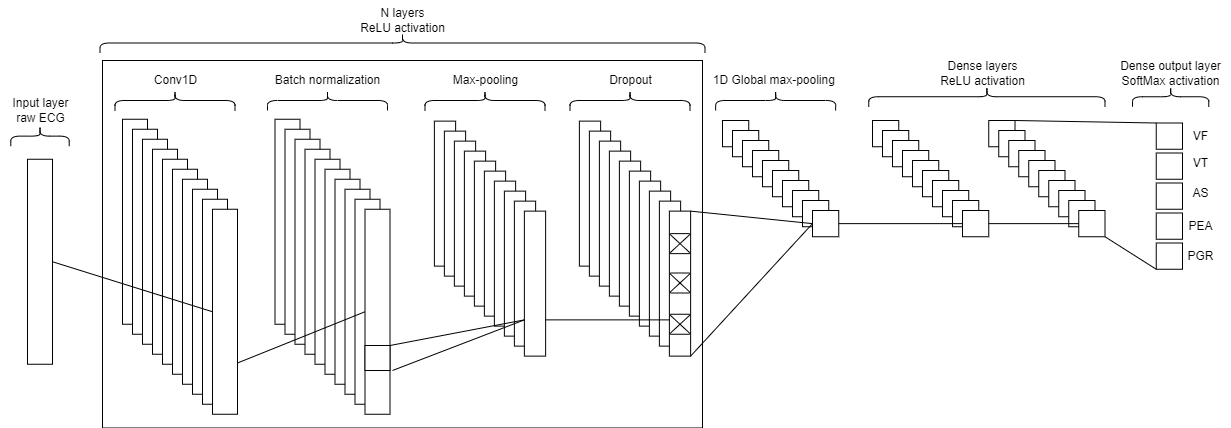
\includegraphics[width=1\linewidth]{Img/CNN_rhythm_classify.png}
    \caption{The structure of the CNN model.}
    \label{fig:CNN_model}
\end{figure}

\subsection{Experiments}\label{subsec:experiments}
When testing the model some of the parameters were set to a fixed value. The batch size was set to 32, learning rate was set to 0.001 and there was a maximum of 250 epochs, with early stopping if the validation loss did not improve for 30 epochs. Additionally the number of fully connected hidden layers was set to two (as described in subsection~\ref{subsec:modelarch}), and the downsampling was done with the pool size set to two.

To test the effect of the different hyperparameters \textit{Keras Tuner} was used to perform random search~\cite{omalley2019kerastuner}. Keras Tuner is a framework with algorithms to find the best parameters for a model. For each N there was done 250 trials, with 10-fold cross validation in each trial. Every trial consist of randomly selected parameters. The parameters which were experimented with are listed below, with $i = 1,2,..,N$ and $j = 1,2$.

\begin{itemize}
    \item N = [2, 3, 4, 5], layers of convolutional blocks in the model.
    \item Dropout: [0.1, 0.2, .., 0.9]
    \item $K_i$ = [5, 10, 15, 20, 25, 30, 40, 50], kernel sizes in Conv1D
    \item $F_i$ = [5, 10, 15, 20, 25, 30, 40, 50], number of filters in Conv1D
    \item $FC_j$ = [16, 32, 64, 128], number of nodes in the fully connected hidden layers 
\end{itemize}

We used Balanced Accuracy (BAC) as our criteria to evaluate the models since the dataset is very unbalanced. Balanced accuracy is a development of the normal accuracy, instead of looking at only how many of the predictions that are correct it looks at how many are correct for each class. This means that it is more accurate for imbalanced datasets~\cite{accuracy}.

$$
\text{BAC} = \frac{\text{Sensitivity} + \text{Specificity}}{2}
$$

After the initial experiments, the dropout and $FC_j$ was fixed, and more experiments were carried out while varying $F_i$ and $K_i$. This time there was done 400 trials for each N.
\section{Results}

The results section is divided in three parts. First the results of the random search without fixed parameters are presented, and then the results with two more of the parameters fixed are presented. At the end of each of these two subsections there is a table that shows the parameters for the most optimal models, and then confusion matrices to summarize the performance of the model.  At last the results from the model giving the highest BAC from the trials is presented, where the results from another 10-fold cross validation training is presented to look at robustness and variation within the model.

\newpage
\subsection{Without fixed parameters}


The scatter plot in figure~\ref{fig:scatter} shows the relation between the accuracy and the number of trainable parameters in the model. The plot to the left uses the accuracy and the plot on the right uses the balanced accuracy. For the rest of the report the results are presented with regards to the BAC.  

From the scatter plot it can be seen that the model does not necessarily improve with added complexity. The BAC does not improve noticeably with more trainable parameters. Since there are five classes, a $BAC=20\%(=\frac{100}{5})$ equals the probability of correctly classifying by random guessing. For $N=5$ there are some number of trainable parameters that makes the BAC go to $20\%$. Why this happens is explained more in the next paragraph. It is not possible to deduce which N works best from this scatter plot, but it is clear that $N=2$ achieves poorer results than the rest.

\begin{figure}[H]
    \centering
    \begin{minipage}[b]{0.48\textwidth}
        \includesvg[width=1\textwidth]{Img/results/unfixed/scatter_acc.svg}
        \vspace{-0.5cm}
    \end{minipage}
    \begin{minipage}[b]{0.48\textwidth}
        \includesvg[width=1\textwidth]{Img/results/unfixed/scatter_bac.svg}
        \vspace{-0.5cm}
    \end{minipage}
    \captionsetup{width=0.95\linewidth}
    \caption{Scatter plots showing the relationship between number of tuneable parameters and the accuracy (on the left) or the balanced accuracy (on the right), for each N. }
    \label{fig:scatter}
\end{figure}

Figure~\ref{fig:dropout_acc} shows the BAC in relation to the dropout for N equal to two, three, four and five. The common factor in all four plots is that a too high dropout value results in a low accuracy. This is what causes the previously mentioned $20\%$ BAC in the scatterplot. For $N=5$ in figure~\ref{fig:dropout_acc} a dropout between $0.7$ and $0.9$ gives this accuracy of $20\%$. When the dropout value gets too high, too many neurons are set to zero, and the model will not have enough information. For all four N the best accuracy is achieved when the dropout median is $0.3$. 

\begin{figure}[H]
    \centering
    \begin{minipage}[b]{0.42\textwidth}
        \includesvg[width=1\textwidth]{Img/results/2_dropout.svg}
        \vspace{-0.5cm}
        \caption*{a)}
    \end{minipage}
    \begin{minipage}[b]{0.42\textwidth}
        \includesvg[width=1\textwidth]{Img/results/3_dropout.svg}
        \vspace{-0.5cm}
        \caption*{b)}
    \end{minipage}
    \begin{minipage}[b]{0.42\textwidth}
        \includesvg[width=1\textwidth]{Img/results/4_dropout.svg}
        \vspace{-0.5cm}
        \caption*{c)}
    \end{minipage}
    \begin{minipage}[b]{0.42\textwidth}
        \includesvg[width=1\textwidth]{Img/results/5_dropout.svg}
        \vspace{-0.5cm}
        \caption*{d)}
    \end{minipage}
    \captionsetup{width=0.95\linewidth}
    \caption{The relationship between dropout and BAC. For a) $N=2$, b) $N=3$, c) $N=4$ and d) $N=5$.}
    \label{fig:dropout_acc}
\end{figure}


The third parameter that was experimented with was the kernel sizes, $K_i$. Figure~\ref{fig:k_acc} shows the relation between kernel size and the accuracy, with one block for each $K_i$. For $N=2$ there seems to be a positive correlation between the two, so that a bigger kernel size yields a better accuracy. For $N>2$ the relation is not as obvious. The kernel size's effect are tested further in the next subsection.


\begin{figure}[H]
    \centering
    \begin{minipage}{0.42\textwidth}
        \includesvg[width=\textwidth]{Img/results/2_ksize.svg}
        \hspace{-0.5cm}
        \caption*{a)}
    \end{minipage}
    \begin{minipage}{0.42\textwidth}
        \includesvg[width=\textwidth]{Img/results/3_ksize.svg}
        \hspace{-0.5cm}
        \caption*{b)}
    \end{minipage}
    \begin{minipage}{0.42\textwidth}
        \includesvg[width=\textwidth]{Img/results/4_ksize.svg}
        \hspace{-0.5cm}
        \caption*{c)}
    \end{minipage}
    \begin{minipage}{0.42\textwidth}
        \includesvg[width=\textwidth]{Img/results/5_ksize.svg}
        \hspace{-0.5cm}
        \caption*{d)}
    \end{minipage}
    \captionsetup{width=0.95\linewidth}
    \caption{The relationship between kernel size and BAC. For a) $N=2$, b) $N=3$, c) $N=4$ and d) $N=5$.}
    \label{fig:k_acc}
\end{figure}

For the number of filters, $F_i$, the relation with the accuracy is shown in figure~\ref{fig:f_acc}. How these two relates to each other is not very obvious from the plots. This parameter was also tested further in the next subsection.

\begin{figure}[H]
    \centering
    \begin{minipage}[b]{0.42\textwidth}
        \includesvg[width=1\textwidth]{Img/results/2_filters.svg}
        \vspace{-0.5cm}
        \caption*{a)}
    \end{minipage}
    \begin{minipage}[b]{0.42\textwidth}
        \includesvg[width=1\textwidth]{Img/results/3_filters.svg}
        \vspace{-0.5cm}
        \caption*{b)}
    \end{minipage}
    \begin{minipage}[b]{0.42\textwidth}
        \includesvg[width=1\textwidth]{Img/results/4_filters.svg}
        \vspace{-0.5cm}
        \caption*{c)}
    \end{minipage}
    \begin{minipage}[b]{0.42\textwidth}
        \includesvg[width=1\textwidth]{Img/results/5_filters.svg}
        \vspace{-0.5cm}
        \caption*{d)}
    \end{minipage}
    \captionsetup{width=0.95\linewidth}
    \caption{The relationship between number of filters and BAC. For a) $N=2$, b) $N=3$, c) $N=4$ and d) $N=5$.}
    \label{fig:f_acc}
\end{figure}

Before the output layers there are two fully connected layers, and the size of these were the last parameter that was experimented with. Figure~\ref{fig:fc_acc} shows the relationship between this size and the accuracy. From this it is possible to take the values with the best accuracy for each N, and this is summarized below. 

\begin{figure}[H]
    \centering
    \begin{minipage}[b]{0.42\textwidth}
        \includesvg[width=1\textwidth]{Img/results/2_fc.svg}
        \vspace{-0.5cm}
        \caption*{a)}
    \end{minipage}
    \begin{minipage}[b]{0.42\textwidth}
        \includesvg[width=1\textwidth]{Img/results/3_fc.svg}
        \vspace{-0.5cm}
        \caption*{b)}
    \end{minipage}
    \begin{minipage}[b]{0.42\textwidth}
        \includesvg[width=1\textwidth]{Img/results/4_fc.svg}
        \vspace{-0.5cm}
        \caption*{c)}
    \end{minipage}
    \begin{minipage}[b]{0.42\textwidth}
        \includesvg[width=1\textwidth]{Img/results/5_fc.svg}
        \vspace{-0.5cm}
        \caption*{d)}
    \end{minipage}
    \captionsetup{width=0.95\linewidth}
    \caption{The relationship between number of nodes in the fully connected hidden layers and BAC. For a) $N=2$, b) $N=3$, c) $N=4$ and d) $N=5$.}
    \label{fig:fc_acc}
\end{figure}

Table~\ref{tab:opt_parameters} shows the parameters for the model that performed best for each N. To assess which model is best, the balanced accuracy was calculated for each model. The BAC is listed on the far right of the table.

\begin{table}[H]
    \centering
    \begin{tabular}{|c|c|c|c|c|c|c|c|c|c|c|c|c|c|c|}
        \hline
        \textbf{N} & \textbf{K1} & \textbf{K2} & \textbf{K3} & \textbf{K4} & \textbf{K5} & \textbf{F1} & \textbf{F2} & \textbf{F3} & \textbf{F4} & \textbf{F5} & \textbf{FC1} & \textbf{FC2} & \textbf{Dropout} & \textbf{Max BAC} \\ \hline
        \textbf{2} & 20 & 50 & - & - & - & 30 & 50 & - & - & - & 64 & 64 & 0.6 & 0.949 \\
        \textbf{3} & 10 & 25 & 50 & - & - & 50 & 20 & 15 & - & - & 128 & 32 & 0.6 & 0.946 \\
        \textbf{4} & 30 & 20 & 50 & 20 & - & 5 & 25 & 40 & 50 & - & 128 & 16 & 0.2 & 0.946 \\
        \textbf{5} & 40 & 40 & 10 & 5 & 20 & 5 & 25 & 40 & 40 & 50 & 64 & 32 & 0.3 & 0.956 \\
        \hline
    \end{tabular}
    \captionsetup{width=0.95\linewidth}
    \caption{Parameters for the most optimal models found under the small random search.}
    \label{tab:opt_parameters}
\end{table}


In figure~\ref{fig:confus} the confusion matrices of the four models in the table are shown. All four models have quite good results, both in terms of the balanced accuracy and the confusion matrices. The model with five convolutional layers has the best results, with $BAC=0.956$ and values on the diagonal of the confusion matrix very close to one.

\begin{figure}[H]
    \centering
    \includesvg[width=0.8\linewidth]{Img/results/unfixed/conf.svg}
    \captionsetup{width=0.95\linewidth}
    \caption{Confusion matrices of the best model for each N.}
    \label{fig:confus}
\end{figure}


\subsection{With fixed parameters}

In this section the dropout and number of nodes in the fully connected layers were fixed, to $Dropout=0.3$, $FC_1=64$ and $FC_2=32$. These experiments where done to try to get a better overview of the effect that kernel size and filters have on the model.

Figure \ref{fig:scatter_fixed} shows the relation between the number of tuneable parameters and the accuracy, for each N. The plot on the left uses accuracy and the plot on the right uses balanced accuracy. It is clear that these results are better than the results without fixed parameters, because none of the models get the BAC of $20\%$. Apart from that one can still observe that more trainable parameters does not necessarily increase the accuracy.

\begin{figure}[H]
    \centering
    \begin{minipage}[b]{0.49\textwidth}
        \includesvg[width=1\textwidth]{Img/results/fixed/scatter_fixed_acc.svg}
        \vspace{-0.5cm}
    \end{minipage}
    \begin{minipage}[b]{0.49\textwidth}
        \includesvg[width=1\textwidth]{Img/results/fixed/scatter_fixed_bac.svg}
        \vspace{-0.5cm}
    \end{minipage}
    \captionsetup{width=0.95\linewidth}
    \caption{Scatter plots showing the relationship between number of trainable parameters and the accuracy (on the left) or the balanced accuracy (on the right), for each N, with fixed parameters.}
    \label{fig:scatter_fixed}
\end{figure}

In figure~\ref{fig:kernel_acc} the relation between the kernel size and the BAC is shown. It is still hard to see any real correlation between kernel sizes and results for the bigger N's, but for $N=2$ and $N=3$ the accuracy gets better for bigger kernel sizes.


\begin{figure}[H]
    \centering
    \begin{minipage}[b]{0.42\textwidth}
        \includesvg[width=1\textwidth]{Img/results/fixed/fixed_2_ksize.svg}
        \vspace{-0.5cm}
        \caption*{a)}
    \end{minipage}
    \begin{minipage}[b]{0.42\textwidth}
        \includesvg[width=1\textwidth]{Img/results/fixed/fixed_3_ksize.svg}
        \vspace{-0.5cm}
        \caption*{b)}
    \end{minipage}
    \begin{minipage}[b]{0.42\textwidth}
        \includesvg[width=1\textwidth]{Img/results/fixed/fixed_4_ksize.svg}
        \vspace{-0.5cm}
        \caption*{c)}
    \end{minipage}
    \begin{minipage}[b]{0.42\textwidth}
        \includesvg[width=1\textwidth]{Img/results/fixed/fixed_5_ksize.svg}
        \vspace{-0.5cm}
        \caption*{d)}
    \end{minipage}
    \captionsetup{width=0.95\linewidth}
    \caption{The relationship between kernel size and BAC with fixed parameters. For a) $N=2$, b) $N=3$, c) $N=4$ and d) $N=5$.}
    \label{fig:kernel_acc}
\end{figure}

The relation between the number of filters and the BAC are plotted in figure~\ref{fig:filter_acc}. This plot does not show any obvious relation between the number of filters and the BAC, so the best number of filters was determined from which model got the best BAC for each N.

\begin{figure}[H]
    \centering
    \begin{minipage}[b]{0.42\textwidth}
        \includesvg[width=1\textwidth]{Img/results/fixed/fixed_2_filters.svg}
        \vspace{-0.5cm}
        \caption*{a)}
    \end{minipage}
    \begin{minipage}[b]{0.42\textwidth}
        \includesvg[width=1\textwidth]{Img/results/fixed/fixed_3_filters.svg}
        \vspace{-0.5cm}
        \caption*{b)}
    \end{minipage}
    \begin{minipage}[b]{0.42\textwidth}
        \includesvg[width=1\textwidth]{Img/results/fixed/fixed_4_filters.svg}
        \vspace{-0.5cm}
        \caption*{c)}
    \end{minipage}
    \begin{minipage}[b]{0.42\textwidth}
        \includesvg[width=1\textwidth]{Img/results/fixed/fixed_5_filters.svg}
        \vspace{-0.5cm}
        \caption*{d)}
    \end{minipage}
    \captionsetup{width=0.95\linewidth}
    \caption{The relationship between number of filters and BAC with fixed parameters. For a) $N=2$, b) $N=3$, c) $N=4$ and d) $N=5$.}
    \label{fig:filter_acc}
\end{figure}

The best models, for each N, found from testing with fixed Dropout and $FC_j$ are listed in table~\ref{tab:opt_parameters2}. The model with the best BAC is highlighted in green, and this is the one that is used in the next subsection. It got a BAC of $0.958$.


\begin{table}[H]
    \centering
    \begin{tabular}{|c|c|c|c|c|c|c|c|c|c|c|c|c|c|}
        \hline
        \textbf{N} & \textbf{K1} & \textbf{K2} & \textbf{K3} & \textbf{K4} & \textbf{K5} & \textbf{F1} & \textbf{F2} & \textbf{F3} & \textbf{F4} & \textbf{F5} & \textbf{Max BAC} \\
        \hline
        \textbf{2} & 40 & 20 & - & - & - & 40 & 20 & - & - & - & 0.942   \\
        \textbf{3} & 25 & 20 & 25 & - & - & 20 & 15 & 30 & - & - & 0.946   \\
        \rowcolor{green}\textbf{4} & 40 & 30 & 10 & 40 & - & 30 & 10 & 25 & 40 & - & 0.958   \\
        \textbf{5} & 40 & 5 & 25 & 25 & 20 & 40 & 15  & 30 & 5 & 10 & 0.946   \\
        \hline
    \end{tabular}
    \caption{Parameters for the optimal models found under random search with fixed parameters: $Dropout=0.3$, and dense layers $FC_1=64$ and $FC_2=32$. With two to five convolution blocks in the models. The green highlights the model with the best BAC.}
    \label{tab:opt_parameters2}
\end{table}

Confusion matrices of the best models for each N are shown in figure~\ref{fig:confus_fix}. This supports the table~\ref{tab:opt_parameters2} in that the model with $N=4$ is the best, as the values on the diagonal are so close to one.

\begin{figure}[H]
    \centering
    \includesvg[width=0.8\linewidth]{Img/results/fixed/conf_fixed.svg}
    \captionsetup{width=0.85\linewidth}
    \caption{Confusion matrices of the best model for each N, with dropout fixed to 0.3, and the fully connected layers fixed at $FC_1 = 64, FC_2 = 32$.}
    \label{fig:confus_fix}
\end{figure}


\subsection{Best model}

To evaluate the best model as found with the fixed random search (green in table~\ref{tab:opt_parameters2}), the model was tested again to see how it performs over 10-fold cross validation.

Figure \ref{fig:best_history} shows all ten training histories when retraining with the best model. From the validation accuracy and the validation loss it is a noticeable difference between each run. 

\begin{figure}[H]
    \centering
    \includesvg[width=0.7\linewidth]{Img/results/best_model/best_training.svg}
    \captionsetup{width=0.95\linewidth}
    \caption{Training histories for all ten runs with the best model.}
    \label{fig:best_history}
\end{figure}

Table~\ref{tab:rp} shows the accuracy, BAC, sensitivity (Sen) and positive predictive value (PPV) for the best model, with median and 25th/75th percentile. The sensitivity is the number of true positives divided by the summation of true positives and false negatives, i.e. it shows if the model can find all objects in the class. The PPV is the number of true positives divided by the summation of true positives and false positives, i.e. it shows how often the model is correct when it predicts this class. The values for ventricular tachycardia (VT) are quite low for both the sensitivity and PPV. This could be because it has a very low number of samples in the training set. The BAC reaches a value of $0.91$, which is a bit lower than in the previous subsection. This can indicate that the model has a lot of variance due to randomness in data selection and weight initialization in the model.

\begin{table}[H]
    \centering
    \begin{tabular}{|c|c|c|c|c|c|c|c|c|c|c|c|c|}
    \hline
         & Acc & BAC & \multicolumn{2}{c|}{AS} & \multicolumn{2}{c|}{PEA} & \multicolumn{2}{c|}{PGR} & \multicolumn{2}{c|}{VF} & \multicolumn{2}{c|}{VT}  \\ \hline
         & & & Sen & PPV & Sen & PPV & Sen & PPV & Sen & PPV & Sen & PPV \\ \hline
         Median & 0.92 & 0.91 & 1.00 & 0.95 & 0.91 & 0.93 & 0.87 & 0.92 & 0.98 & 0.95 & 0.82 & 0.74 \\ \hline
         25th percentile & 0.91 & 0.91 & 0.98 & 0.95 & 0.90 & 0.92 & 0.86 & 0.92 & 0.97 & 0.93 & 0.78 & 0.69 \\ \hline
         75th percentile & 0.93 & 0.92 & 1.00 & 0.95 & 0.92 & 0.94 & 0.88 & 0.94 & 0.98 & 0.96 & 0.82 & 0.76 \\ \hline
    \end{tabular}
    \caption{Table containing the median and the 25th/75th percentile of accuracy, BAC, sensitivity (Sen) and positive predictive value (PPV) of every class when retesting the "best model".}
    \label{tab:rp}
\end{table}


% \begin{table}[H]
%     \centering
%     \begin{tabular}{|c|c|}
%         \hline
%             & Median (25th percentile, 75th percentile) \\
%         \hline
%         Acc & 0.92 (0.91, 0.93) \\
%         BAC & 0.91 (0.91, 0.92) \\
%         \hline
%         AS (Sen) & 1.00 (0.98, 1.00) \\
%         AS (P) & 0.95 (0.95, 0.95) \\
%         \hline
%         PEA (Sen) &  0.91 (0.90, 0.92) \\
%         PEA (P) &  0.93 (0.92, 0.94) \\
%         \hline
%         PGR (Sen) & 0.87 (0.86, 0.88) \\
%         PGR (P) & 0.92 (0.92, 0.94) \\
%         \hline
%         VF (Sen) & 0.98 (0.97, 0.98) \\
%         VF (P) & 0.95 (0.93, 0.96) \\
%         \hline
%         VT (Sen) & 0.82 (0.78, 0.82) \\
%         VT (P) & 0.74 (0.69, 0.76) \\
%         \hline
%     \end{tabular}
%     \caption{Table containing the median and the 25th/75th percentile of accuracy, BAC, sensitivity (Sen) and precision (P) of every class when retesting the "best model".}
%     \label{tab:rp}
% \end{table}


\section{Discussion}

In general this type of network seems to work well for classifying heart rhythms, with many of the models reaching over $90\%$ BAC. This section will discuss the outcome of the project and some areas where there is potential for improvement.


%
To achieve more robust and better results, a larger dataset could be desirable. There does not exist a specific rule that says how big a dataset should be for a CNN, but most sources agree that it should be as big as possible. Also, as mentioned in section~\ref{sec:matandmet}, the balance of the dataset could be better. Especially the VT samples are very few, and this leads to the model having a harder time classifying this class correctly. 

With the current model architecture it was not possible to have more than five convolution blocks. This is because most trials would fail with more convolution blocks due to the down-sampling. A possible improvement is to have smaller kernels in the later layers, and/or use padding with the max pooling layers. This would make it possible to have more convolution blocks.

Future work could also experiment more with the fully connected layers. This was not experimented much with, and as~\cite{fullyconnected} says, bigger fully connected layers probably would improve the model. There could also be made a few improvements to how the parameters are tested. Often the size of both filter and kernels gets smaller for each layer, while in this model the size was chosen randomly. 

\subsection{Conclusion}

This project has developed a CNN model for classifying heart rhythms. It has been tested, first with five non-fixed parameters and then with three. The best model was achieved with four convolutional blocks, which gave a balanced accuracy of $0.91$. The biggest improvements to the model from the previous project~\cite{cardiac}, is the added global max pooling after the convolutional blocks, and bigger kernel sizes in the convolutional layer. This resulted in a more robust model with less overfitting and better test results. 

The same dataset is used in the articles "A Convolutional Neural Network Approach for Interpreting Cardiac Rhythms from Resuscitation of Cardiac Arrest Patients"~\cite{eftes} and "Multimodal Biosignal Analysis Algorithm for the  Classification of Cardiac Rhythms During Resuscitation"~\cite{lasa}. Compared to the results from these articles, this project has achieved improvements in Acc, Sen and PPV. This can especially be seen in the Sen and PPV of the VT class. Where in the first article Sen = 0.60 and PPV = 0.481, the second Sen = 0.773 and PPV = 0.661, and in this project Sen = 0.82 and PPV = 0.74. This shows that the project have made progress in the study of classifying heart rhythms.  
 



%\newpage
%Referanser

\renewcommand{\bibname}{References}
\bibliography{references.bib}
%\nocite{*}

\end{document}   

